\documentclass[12pt]{article}
\usepackage{cite}
\usepackage{graphicx}
\usepackage{geometry}
\usepackage{float}
\usepackage{multicol}
\usepackage{subfigure}

\geometry{left=2.0cm,right=2.0cm,top=2.5cm,bottom=2.5cm}

\title{
    \textbf{\Huge ECE385} \\
    \huge Fall 2020 \\
    \huge Experiment 7 \\[120pt]
    \textbf{\Huge SOC with NIOS-II in SystemVerlog} \\[120pt]
    }

\author{
    \large Name: Zhou Qinren \\ 
            \quad\qquad Zhang Yichi \\
    \large Lab Section: LA3 \\
    \large TA's Name: Yu Yuqi
    }

\date{Nov. $17^{th}$ 2020}

\begin{document}
\setlength{\parindent}{0pt}
\maketitle
\newpage

\section{Introduction}
In this lab, we build a system on chip (SoC) with NIOS-II processor using the platform designer. We work on the eclipse for the first time to write, compile and execute C codes on the FPGA connecting software and hardware and implementing LED blink and accumulator.

\section{Written Description and Diagrams of NIOS-II System}
The hardware component of this lab includes the NIOS-II processor and its peripherals. The NIOS-II processor works as a CPU that stores temporary data, do the basic arithmetics and execute instructions. It connects to the SDRAM controller to manage the data transfer with the SDRAM and the SDRAM PLL to phase shift the external clock to provide a precise clock signal for the SDRAM. Also, it connects to the PIOs to control hardware inputs and outputs such as LEDs, switches and Keys.

\section{Top Level Block Diagram}
\begin{figure}[H]
    \centering
    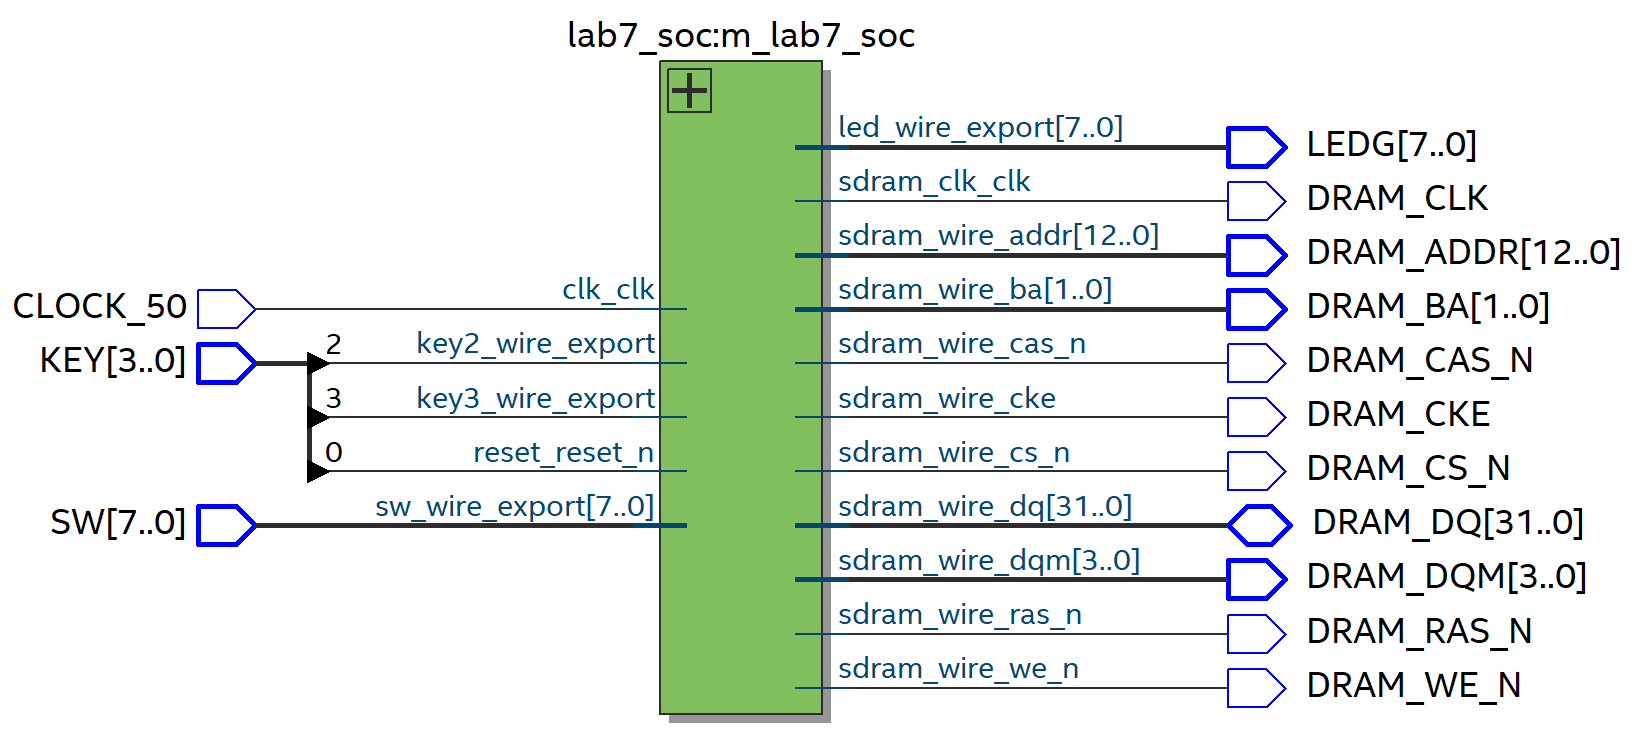
\includegraphics[width=16cm]{top.png}
    \caption{Top level block diagram.}
\end{figure}

\section{Written Description of all .sv Modules}
\textbf{Module}: lab7\_soc \\ 
\textbf{Inputs}: clk\_clk, key2\_wire\_export, key3\_wire\_export, reset\_reset\_n, sw\_wire\_export \\ 
\textbf{Outputs}: [7:0] led\_wire\_export, sdram\_clk\_clk, [12:0] sdram\_wire\_addr, [1:0] sdram\_wire\_ba, sdram\_wire\_cas\_n, sdram\_wire\_cke, sdram\_wire\_cs\_n, [3:0] sdram\_wire\_dqm, sdram\_wire\_ras\_n, sdram\_wire\_we\_n \\ 
\textbf{Inouts}: [31:0] sdram\_wire\_dq \\
\textbf{Description}: This is the whole system on chip module generated by platform designer that connects all the hardware together. \\ 
\textbf{Purpose}: This SoC module provide us a hardware environment to build software on. It takes in the inputs from the clock, switches and keys and outputs the result through the wires to the SDRAM and LEDs. \\

\textbf{Module}: lab7 \\ 
\textbf{Inputs}: CLOCK\_50, [3:0] KEY, [7:0] SW \\ 
\textbf{Outputs}: [7:0] LEDG, [12:0] DRAM\_ADDR, [1:0] DRAM\_BA, DRAM\_CAS\_N, DRAM\_CKE, DRAM\_CS\_N, [3:0] DRAM\_DQM, DRAM\_RAS\_N, DRAM\_WE\_N, DRAM\_CLK \\ 
\textbf{Inouts}: [31:0] DRAM\_DQ \\
\textbf{Description}: This is the top level module. \\ 
\textbf{Purpose}: This module connects the real LEDs, switches, keys and DRAM to the SoC module.

\section{System Level Block Diagram}
\begin{figure}[H]
    \centering
    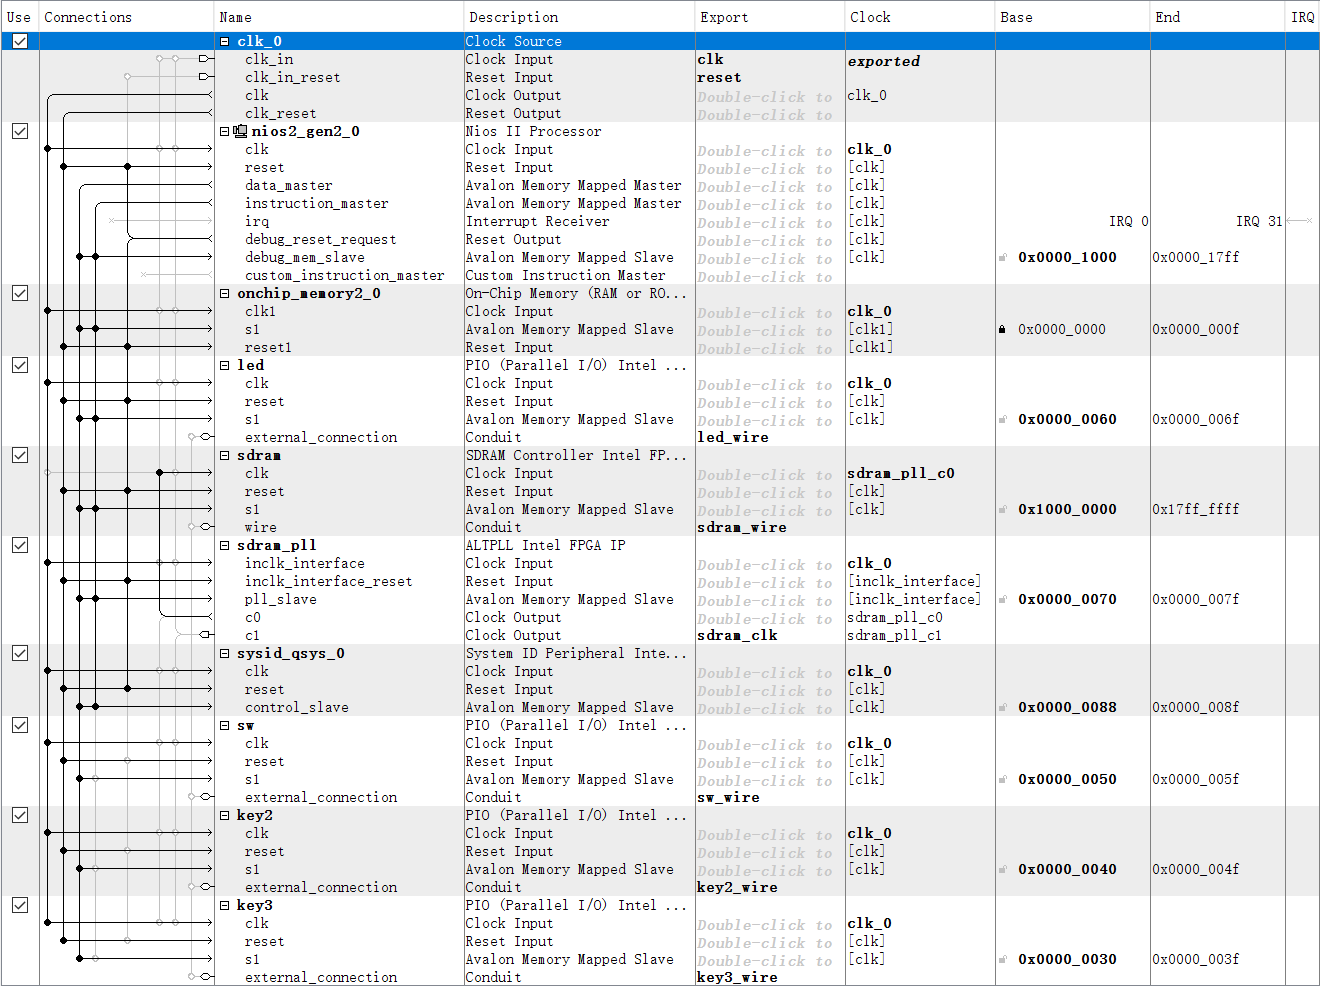
\includegraphics[width=15cm]{platform.png}
    \caption{Platform Designer view.}
\end{figure}

\textbf{block}: clk\_0 \\
\textbf{Inputs}: clk\_in, clk\_in\_reset \\
\textbf{Outputs}: clk, clk\_reset \\
\textbf{functionality}: The clock of all the components of SoC except for the SDRAM controller. \\

\textbf{block}: nios2\_gen2\_0 \\
\textbf{Inputs}: clk, reset, debug\_mem\_slave \\
\textbf{Outputs}: data\_master, instruction\_master, debug\_reset\_request \\
\textbf{functionality}: NIOS-II processor, the CPU. \\

\textbf{block}: onchip\_memory2\_0 \\
\textbf{Inputs}: clk1, s1, reset1 \\
\textbf{functionality}: An onchip memory storing temorary data like a Regfile in lc3.

\textbf{block}: led \\
\textbf{Inputs}: clk, reset, s1 \\
\textbf{functionality}: LED. \\

\textbf{block}: sdram \\
\textbf{Inputs}: clk, reset, s1 \\
\textbf{functionality}: SDRAM controller. It interfaces and transfers data with the SDRAM chip. \\

\textbf{block}: sdram\_pll \\
\textbf{Inputs}: inclk\_interface, inclk\_interface\_reset, pll\_slave \\
\textbf{Outputs}: c0, c1 \\
\textbf{functionality}: The clock for SDRAM controller and the clock for SDRAM. \\

\textbf{block}: sysid\_qsys\_0 \\
\textbf{Inputs}: clk, reset, control\_slave \\
\textbf{functionality}: System ID. It ensures the compatibility between hardware and software. \\

\textbf{block}: sw \\
\textbf{Inputs}: clk, reset, s1 \\
\textbf{functionality}: Switch inputs. \\

\textbf{block}: key2 \\
\textbf{Inputs}: clk, reset, s1 \\
\textbf{functionality}: Key[2] input for reset. \\

\textbf{block}: key3 \\
\textbf{Inputs}: clk, reset, s1 \\
\textbf{functionality}: Key[3] input for accumulating. \\

\section{Software Component}
\begin{figure}[H]
    \centering
    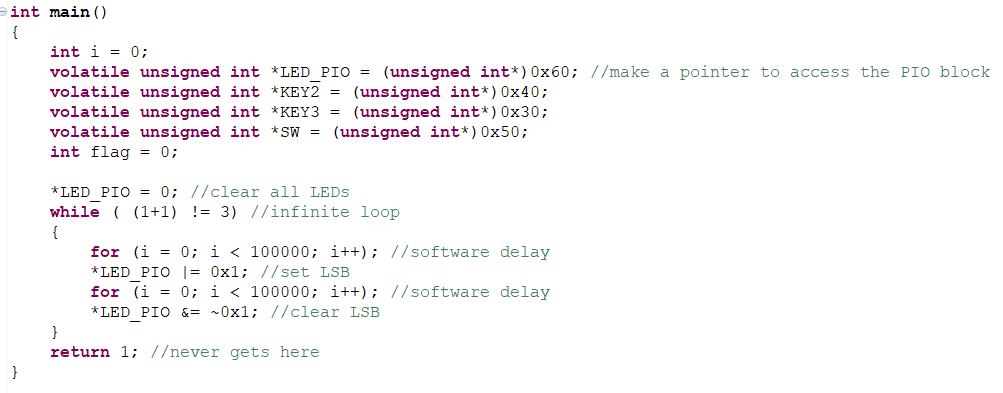
\includegraphics[width=16cm]{LED_blink.png}
    \caption{Codes for LED blink.}
\end{figure}
This is the code for LED blink. We use for loop to simulate the delay, so every 100000 loops we turn on or turn off the LED.

\begin{figure}[H]
    \centering
    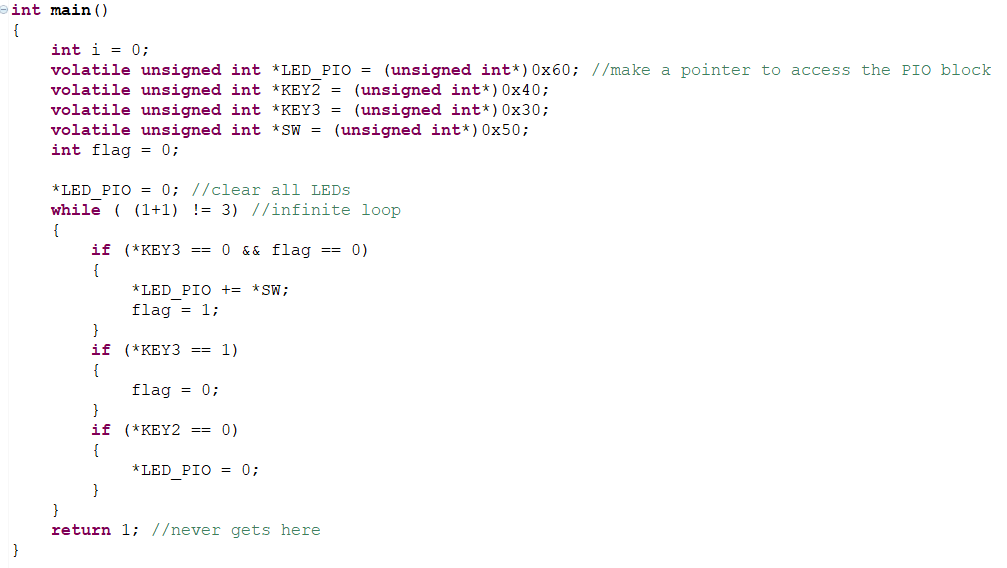
\includegraphics[width=16cm]{Accumulator.png}
    \caption{Codes for accumulator.}
\end{figure}
This is the code for accumulator. Every time the Key3 is pressed, we add the value represented by switches to the LED so the corresponding LEDs light up and set the flag to 1 to prevent unwanted accumulation when we press the key for a long time. The flag will be reset to 0 until we release the key3. When we press key2, we reset the LEDs.

\section{Answers to all 11 INQ Questions}
Question: What are the differences between the Nios II/e and Nios II/f CPUs? \\

Answer: Nios II/e is the economy version of the processor, it has less functionalities than Nios II/f, but it takes up less places and resources. \\

Question: What advantage might on-chip memory have for program execution? \\

Answer: The transmission time may be much shorter, i.e., the write and read operations are more efficient, since the memory is allocated on chip, rather than somewhere far away such as sdram. \\

Question: Note the bus connections coming from the NIOS II; is it a Von Neumann, “pure Harvard”, or “modified Harvard” machine and why? \\

Answer: It is a modified Harvard machine. Because the instruction memory may be accessed as data. \\

Question: Note that while the on-chip memory needs access to both the data and program bus, the led peripheral only needs access to the data bus. Why might this be the case? \\

Answer: The reason is that the led only needs data so that it can output the corresponding information. LED does not run the program. \\

Question: Why does SDRAM require constant refreshing? \\

Answer: Because SDRAM has to preserve the contents, otherwise the charges in the capacitor may leak out, and the information may be lost. \\

Question: make sure this is consistent with your above numbers; you will need to justify how you came up with 1 Gbit to your TA. \\

Answer: $32 bits * 2^{13} * 2^{10} * 4 * 2 = 1 Gbit$ \\

Question: What is the maximum theoretical transfer rate to the SDRAM according to the timings given? \\

Answer: 1 / 5.5ns * 32bit = 5.42Gbit /s \\

Question: The SDRAM also cannot be run too slowly (below 50 MHz). Why might this be the case? \\

Answer: The reason might be that the refresh rate is too slow, and the charge leaks out, resulting in data corruption. \\

Question: This puts the clock going out to the SDRAM chip (clk c1) 3ns behind of the controller clock (clk c0). Why do we need to do this? \\

Answer: SDRAM requires a precise clock. We have to compensate for the delay due to transmission or other reasons. \\

Question: What address does the NIOS II start execution from? Why do we do this step after assigning the addresses? \\

Answer: The program starts from address 0x10000000, which is the reset vector. \\

Question: Look at the various segment (.bss, .heap, .rodata, .rwdata, .stack, .text), what does each section mean? Give an example of C code which places data into each segment. \\


Answer: \\
.bss:		a global variable not initialized to a specific value \\
Code:		int i; \\

.heap:		memory which is allocated on heap \\
Code:		int *ptr = (int*)malloc(sizeof(int)); \\

.rodata: 	read only data, const \\
Code:		const int i = 3; \\

.rwdata:	read and write data \\
Code:		int i = 3; \\


.stack:		stack which implements function call \\
Code:		i = foo(parameter); \\

.text:		string segment \\
Code:		char[] str = “hello world”; \\

\section{Postlab Question}
\begin{table}[H]
    \centering
    \resizebox*{9cm}{5cm}{
        \begin{tabular}{|l|l|l|l|}
        \hline
        SDRAM Parameter    & Value    \\ \hline
        Data width         & 32       \\ \hline
        \# of Rows         & 13       \\ \hline
        \# of Columns      & 10       \\ \hline
        \# of Chip selects & 1        \\ \hline
        \# of Banks        & 4        \\ \hline
        \end{tabular}
    }
    \caption{SDRAM parameter.}
\end{table}

\begin{table}[H]
    \centering
    \resizebox*{9cm}{6cm}{
        \begin{tabular}{|l|l|l|l|}
        \hline
        LUT           & 2222       \\ \hline
        DSP           & 0          \\ \hline
        BRAM          & 36864      \\ \hline
        Flip-Flop     & 1960       \\ \hline
        Frequency     & 79.21MHz   \\ \hline
        Static Power  & 102.03mW   \\ \hline
        Dynamic Power & 39.97mW    \\ \hline
        Total Power   & 195.41mW   \\ \hline
        \end{tabular}
    }
    \caption{Design statistics table for the multiplier.}
\end{table}

\section{Conclusion}
This lab is easy to conduct but it takes much time to digest the information. We had little trouble during the lab. 

\newpage
\bibliography{}
\bibliographystyle{ieeetr}
\end{document}